\documentclass[hidelinks,12pt]{article}
\usepackage[round]{natbib}
\usepackage{diagbox} 
\usepackage{multirow}
\usepackage{xcolor}
\bibliographystyle{plainnat}
\usepackage{amsmath}
\usepackage{amssymb}
\usepackage{graphicx}
\usepackage{geometry}
\usepackage{wrapfig}
\usepackage{subcaption}
\usepackage{float}
\geometry{scale = 0.85}
\usepackage{fancyhdr}
\usepackage{hyperref}

\rhead{
\includegraphics[scale=0.3]{logo}}
\begin{document}
\title{CZ2007 LAB 3\\
\large INTRODUCTION TO DATABASE}
\date{}
\author{
    Zou Zeren U2022422H\\
    Zeng Xunyi U2022509A\\
    Tan Pei Lun U2022841A\\
    Bryan Chatsirichai U2022154D\\
    Mulder Choo U2022324D
}
\maketitle\thispagestyle{fancy}
\newpage

\tableofcontents
\newpage
\begin{enumerate}
    \section{CREDIT\_CARD}
    \item[] CREDIT\_CARD (card\_num, bank, date\_valid\_to, date\_valid\_from, customer\_id) 
    \begin{description}
        \item[Keys:] card\_num
        \item[Primary Key:] card\_num
        % \item[Foreign Keys:] customer\_id \textbf{references} CUSTOMER
        \item[FDs:] card\_num $\rightarrow$  bank, date\_valid\_to, date\_valid\_from,customer\_id
        \item All the attributes  are functionally dependent on solely the Primary Key (card\_num)
        \item $\therefore$ The relation is in 3NF 
    \end{description}



\section{CUSTOMER} CUSTOMER (customer\_id, username, email,password,full\_name,address,phone\_num) 
    \begin{description}
        \item[Keys:] customer\_id,username, email
        \item[Primary Key:] customer\_id
       % \item[Foreign Keys:] none
        \item[FDs:]
        \item customer\_id $\rightarrow$  username, email,password, full\_name,address,phone\_num
        \item username $\rightarrow$ customer\_id , email,password, full\_name,address,phone\_num
        \item email $\rightarrow$  username, customer\_id,password, full\_name,address,phone\_num
        \item phone\_num $\rightarrow$full\_name, address
        \item $\therefore$The relation is \textbf{not}  in 3NF 
        \item   
        \item[3NF Procedures:]
        \item[Mninimal Basis for R:]
        \item CUSTOMER (customer\_id(A), username(B), email(C),password(D),full\_name(E),\\address(F),phone\_num(G)) 
        \item = CUSTOMER(A,B,C,D,E,F,G)
        \item[KEYS:]A,B,C
        \item[FDS:]A$\rightarrow$BCDEFG,\ B$\rightarrow$ACDEFG,\ C$\rightarrow$BADEFG \\ ,\ G$\rightarrow$EF
        \item[STEP 1:]
        \item A$\rightarrow$B,\ A$\rightarrow$C,\ A$\rightarrow$D,\ A$\rightarrow$E,\ A$\rightarrow$F,\ A$\rightarrow$G
        \item B$\rightarrow$A,\ B$\rightarrow$C,\ B$\rightarrow$D,\ B$\rightarrow$E,\ B$\rightarrow$F,\ B$\rightarrow$G
        \item C$\rightarrow$A,\ C$\rightarrow$B,\ C$\rightarrow$D,\ C$\rightarrow$E,\ C$\rightarrow$F,\ C$\rightarrow$G
        \item G$\rightarrow$E,\ G$\rightarrow$F                                                                                                                                                                                                                                                                                                                             
        \item[STEP 2:] 
        \item we remove 
        \item B$\rightarrow$A,\ B$\rightarrow$C,\ B$\rightarrow$D,\ B$\rightarrow$E,\ B$\rightarrow$F,\ B$\rightarrow$G
        \item C$\rightarrow$A,\ C$\rightarrow$B,\ C$\rightarrow$D,\ C$\rightarrow$E,\ C$\rightarrow$F,\ C$\rightarrow$G
        \item A$\rightarrow$E,\ A$\rightarrow$F
        \item $\{A\}^+$=\{ABCDEFG\}
        \item A$\rightarrow$B,\quad A$\rightarrow$C,\quad A$\rightarrow$D,\quad A$\rightarrow$G,\quad G$\rightarrow$E,\quad G$\rightarrow$F
        \item
        \item $\therefore$  B$\rightarrow$A,\ B$\rightarrow$C,\ B$\rightarrow$D,\ B$\rightarrow$E,\ B$\rightarrow$F,\ B$\rightarrow$G
        \item C$\rightarrow$A,\ C$\rightarrow$B,\ C$\rightarrow$D,\ C$\rightarrow$E,\ C$\rightarrow$F,\ C$\rightarrow$G
        \item A$\rightarrow$E,\ A$\rightarrow$F is redundant
        \item 
        \item[STEP 3:]No FD have redundant attributes on LHS
        \item A$\rightarrow$B,\quad A$\rightarrow$C,\quad A$\rightarrow$D,\quad A$\rightarrow$G
        \item G$\rightarrow$E,\quad G$\rightarrow$F
        \item 
        \item[3NF:]
        \item A$\rightarrow$BCDG \quad G$\rightarrow$EF  
        \item $R_1$ (ABCDG)\quad =\quad  $R_1$ (customer\_id, username, email,password,phone\_num)
        \item $R_2$ (GEF)\quad  = \quad   $R_2$(phone\_num,full\_name,address)
        \item $\therefore$ The relation is in 3NF 
    \end{description}


\newpage

\section{ORDER} ORDER (order\_id, date, status, customer\_id)   
\begin{description}
    \item[Keys:] order\_id
    \item[Primary Key:] order\_id
    %\item[Foreign Keys:] customer\_id \textbf{references} CUSTOMER
    \item[FDs:] order\_id $\rightarrow$ date, status, customer\_id
    \item All the attributes  are functionally dependent on solely the Primary Key (order\_id)
    \item $\therefore$The relation is in 3NF 
\end{description}

\section{ORDER\_ITEM} ORDER\_ITEM ( sequence\_num(A), order\_id(B), product\_unit\_price(C), quantity(D), status(E),
                    \\product\_id(F), shipment\_id(G)) 
\begin{description}
    \item[Keys:] \{sequence\_num(A), order\_id(B)\}
    \item[Primary Key:] \{sequence\_num(A), order\_id(B)\}
    \item[FDs:]  AB$\rightarrow$CDEFG \quad F$\rightarrow$C
    \item[] F$\rightarrow$C violates 3NF (F is not a superkey, C is not contained in a key) 
    \item[Step 1:] Find minimal Basis
    \begin{enumerate}
    \item [Step 1.1] (Keep RHS only 1 attribute): 
    \item [] AB$\rightarrow$C,\quad AB$\rightarrow$D,\quad AB$\rightarrow$E, \quad AB$\rightarrow$F,\quad AB$\rightarrow$G,F$\rightarrow$C
    \item [Step 1.2] (Remove redundant FD):
    \item [] AB$\rightarrow$D, \quad AB$\rightarrow$E, \quad AB$\rightarrow$F,\quad AB$\rightarrow$G, \quad F$\rightarrow$C
    \item [Step 1.3] (Remove dedundanr attributes on LHS):
    \item [] AB$\rightarrow$D,\quad AB$\rightarrow$E, \quad AB$\rightarrow$F,\quad AB$\rightarrow$G,\quad F$\rightarrow$C
    \end{enumerate}
    \item[Step 2:] Combine FDs whose LHS are same):
    \item[] AB$\rightarrow$DEFG, \quad F$\rightarrow$C
    \item[Step 3:] Create a table for each FD: 
    \item[] $R_1$(A, B, D, E, F, G),\quad $R_2$(F,C)  
    % \item[Step 4:] $R_2$(F,C) is redundant with PRODUCT table, so we need to remove $R_2$
    % \item[] $\therefore$ Final Answer:  R(A, B, D, E, F, G)
    % \item[]  
    % \item[] ORDER\_ITEM ( sequence\_num(A), order\_id(B), quantity(D), status(E),
    % product\_id(F), \\shipment\_id(G)) 
    % \item[] All the attributes  are functionally dependent on solely its 
    % \item[] Primary Key\{sequence\_num(A), order\_id(B)\}
     \item[]
     \item $\therefore$The relation is in 3NF 
\end{description}

\newpage





\section{PRODUCT\_TYPE} PRODUCT\_TYPE (product\_type\_id, description, parent\_product\_type\_id) 
\begin{description}
    \item[Keys:] product\_type\_id
    \item[Primary Key:] product\_type\_id
 % \item[Foreign Keys:] parent\_product\_type\_id \textbf{references} PRODUCT\_TYPE
    \item[FDs:] product\_type\_id $\rightarrow$ description, parent\_product\_type\_id 
    \item All the attributes  are functionally dependent on solely its Primary Key(product\_type\_id)
    \item $\therefore$The relation is in 3NF 
\end{description}


\section{RESTRICTED\_TO} RESTRICTED\_TO (shop\_id, product\_type\_id)  
\begin{description}
    \item[Keys:] \{shop\_id,product\_type\_id\}
    \item[Primary Key:] \{shop\_id,product\_type\_id\}
    %\item[Foreign Keys:] product\_type\_id \textbf{references} PRODUCT\_TYPE
    \item[FDs:] shop\_id,product\_type\_id $\rightarrow$  shop\_id,product\_type\_id
    \item Only trival FD exists in the relation
    \item $\therefore$ The relation is in 3NF 
\end{description}


\section{SHIPMENT} SHIPMENT (shipment\_id, tracking\_num, date) 
\begin{description}
    \item[Keys:] shipment\_id, tracking\_num
    \item[Primary Key:] shipment\_id
   % \item[Foreign Keys:]  invoice\_number \textbf{references} INVOICE
    \item[FDs:] shipment\_id $\rightarrow$  tracking\_num, date \quad 
    \item[] tracking\_num $\rightarrow$ shipment\_id, date
    \item All the attributes  are functionally dependent on solely its Primary Key(shipment\_id) 
    \item $\therefore$The relation is in 3NF 
\end{description}

\section{INVOICE} INVOICE(invoice\_number,date,status,order\_id)
\begin{description}
    \item[Keys:] invoice\_number
    \item[Primary Key:] invoice\_number
    %\item[Foreign Keys:]  order\_id \textbf{references} ORDER
    \item[FDs:] invoice\_number $\rightarrow$  date,status,order\_id
    \item All the attributes  are functionally dependent on solely its Primary Key(invoice\_number) 
    \item $\therefore$The relation is in 3NF 
\end{description}

\section{PAYMENT} PAYMENT (payment\_id, amount, card\_num,invoice\_number) 
\begin{description}
    \item[Keys:] payment\_id
    \item[Primary Key:] payment\_id
   %\item[Foreign Keys:] card\_num,invoice\_number \textbf{references} 
    \item[FDs:] payment\_id  $\rightarrow$  amount,card\_num,invoice\_number
    \item All the attributes  are functionally dependent on solely its Primary Key(payment\_id) 
    \item $\therefore$The relation is in 3NF 
\end{description}


\section{PRODUCT} PRODUCT(product\_id,name,colour,price,size,description,shop\_id,product\_type\_id)

\begin{description}
    \item[Keys:] product\_id
    \item[Primary Key:] product\_id
   % \item[Foreign Keys:]
   % \item shop\_id \textbf{references}  SHOP
  %  \item product\_type\_id \textbf{references}  PRODUCT\_TYPE
    \item[FDs:] product\_id $\rightarrow$ name,colour,price,size,description,shop\_id,product\_type\_id
    \item All the attributes  are functionally dependent on solely its Primary Key(payment\_id)
    \item $\therefore$The relation is   in 3NF 
\end{description}



\section{PRODUCT\_PHOTO} PRODUCT\_PHOTO(photo\_sequence,product\_id,pic)

\begin{description}
    \item[Keys:] \{photo\_sequence, product\_id\}
    \item[Primary Key:] \{photo\_sequence,product\_id\}
   % \item[Foreign Keys:]  product\_id \textbf{references}  PRODUCT
    \item[FDs:] photo\_sequence,product\_id $\rightarrow$ pic
    \item All the attributes  are functionally dependent on solely its \\Primary Key ( photo\_sequence,product\_id\ )
    \item $\therefore$The relation is   in 3NF 
\end{description}

\newpage

\section{SHOP} SHOP (shop\_id, shop\_name)
\begin{description}
    \item[Keys:] shop\_id
    \item[Primary Key:] shop\_id
  %  \item[Foreign Keys:] none
    \item[FDs:] shop\_id$\rightarrow$ shop\_name
    \item     \item All the attributes  are functionally dependent on solely its \\Primary Key ( shop\_id ) 
    \item $\therefore$The relation is in 3NF 
\end{description}


\section{ERD REFERENCE}
\qquad\qquad\qquad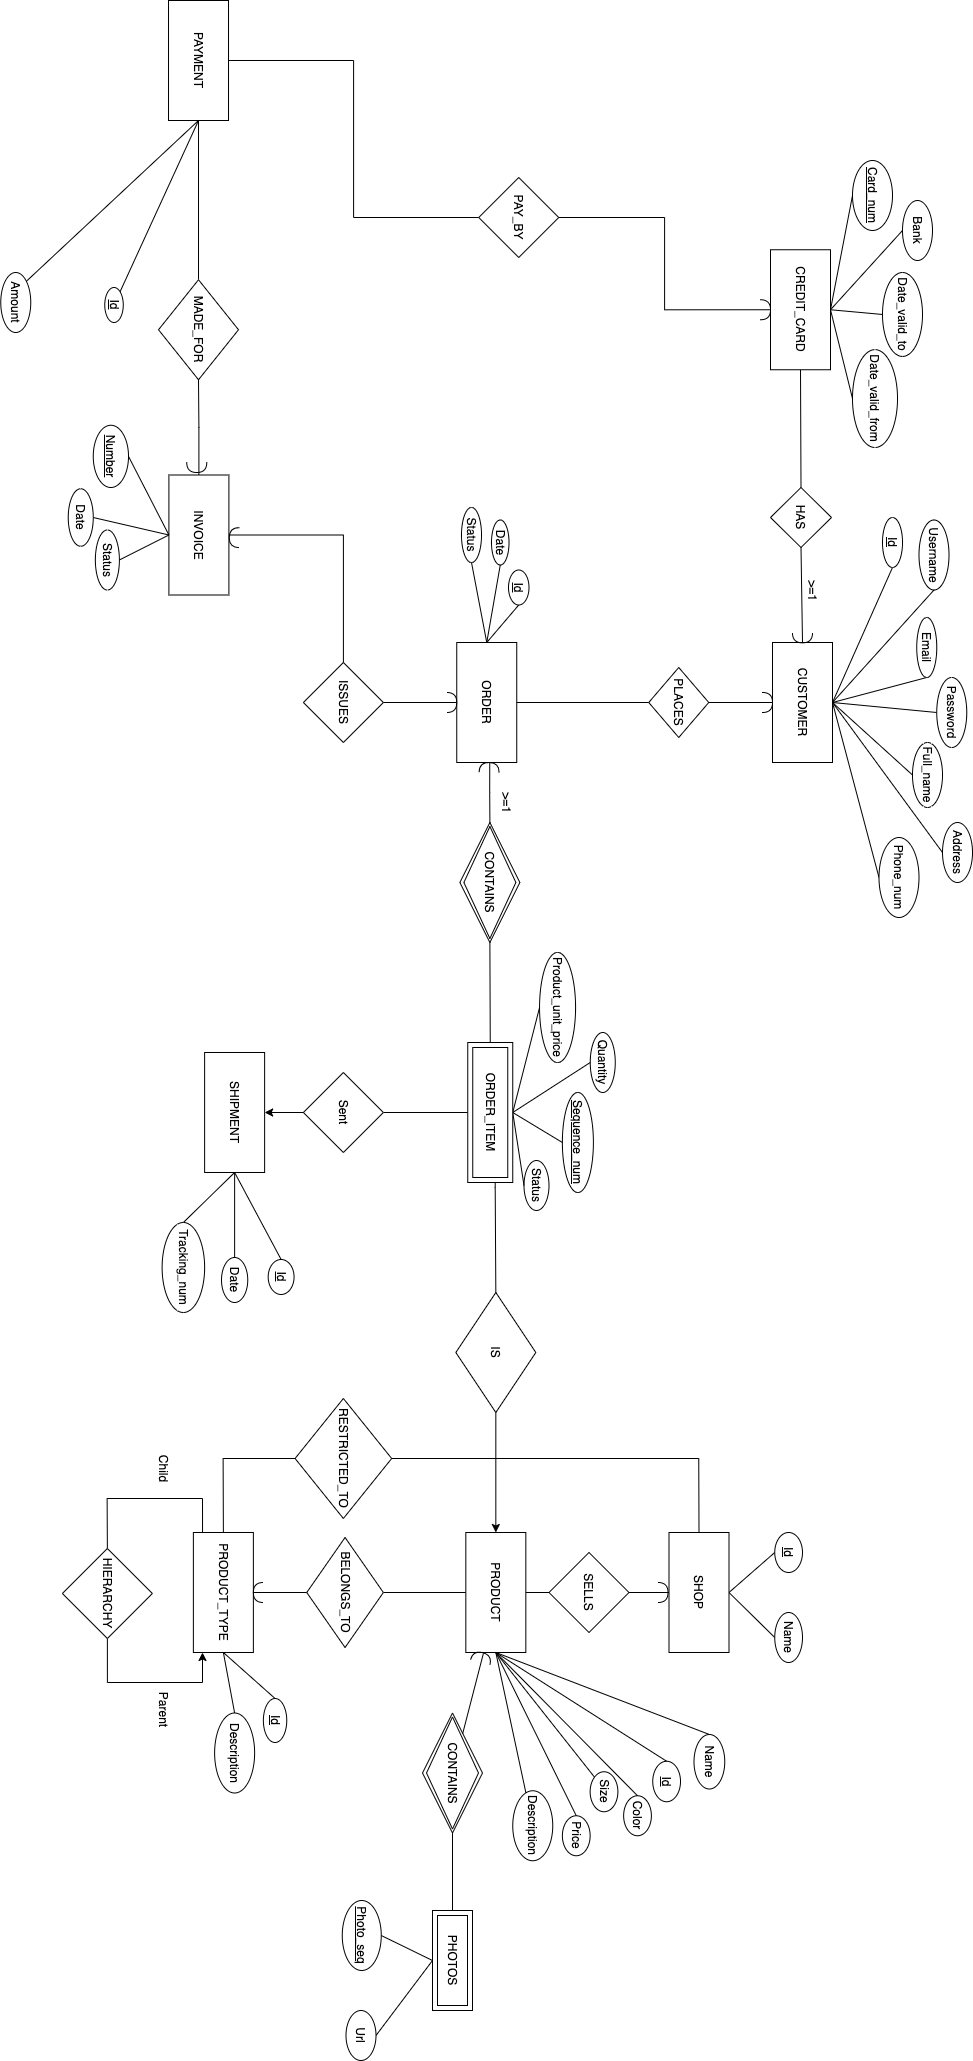
\includegraphics[width=0.583\columnwidth]{ERD_1.4.png}
\end{enumerate}



\end{document}